% Alloy analysis, to be included in alloy.tex

\newpage
\subsection{Alloy analysis}
\label{sect:run}
As a proof of consistency, the following commands were run, thus obtaining the results in Figure \ref{run}.

\begin{lstlisting}[language=alloy]
	run canEnter for 5 but 7 Int
	check noEnterIfFull for 5 but 7 Int
	check noWrongState for 5 but 7 Int
	run showOneTicketPerState for 5 but 7 Int, exactly 1 Store
\end{lstlisting} 

\begin{figure}[h]
	\centering	
	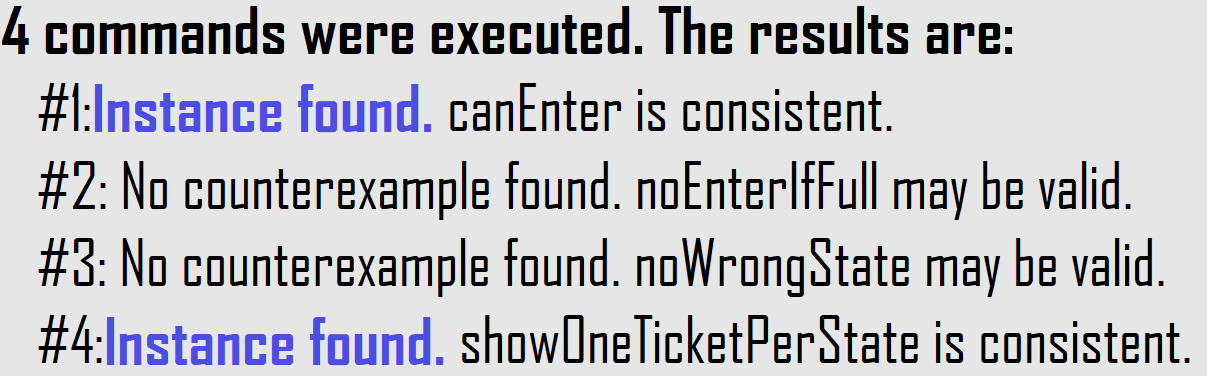
\includegraphics[width=0.6\textwidth] {alloy/alloyrun}
	\caption{Alloy analysis results}
	\label{run} 
\end{figure}

The generated world can be seen in Figure \ref{metamodel}, while Figure \ref{oneforstate} offers an example where exists a ticket for each consistent state (Non-relevant signatures are hidden in Figure \ref{oneforstate_compl}).

\begin{landscape}
	\begin{figure}[p]	
		\centering
		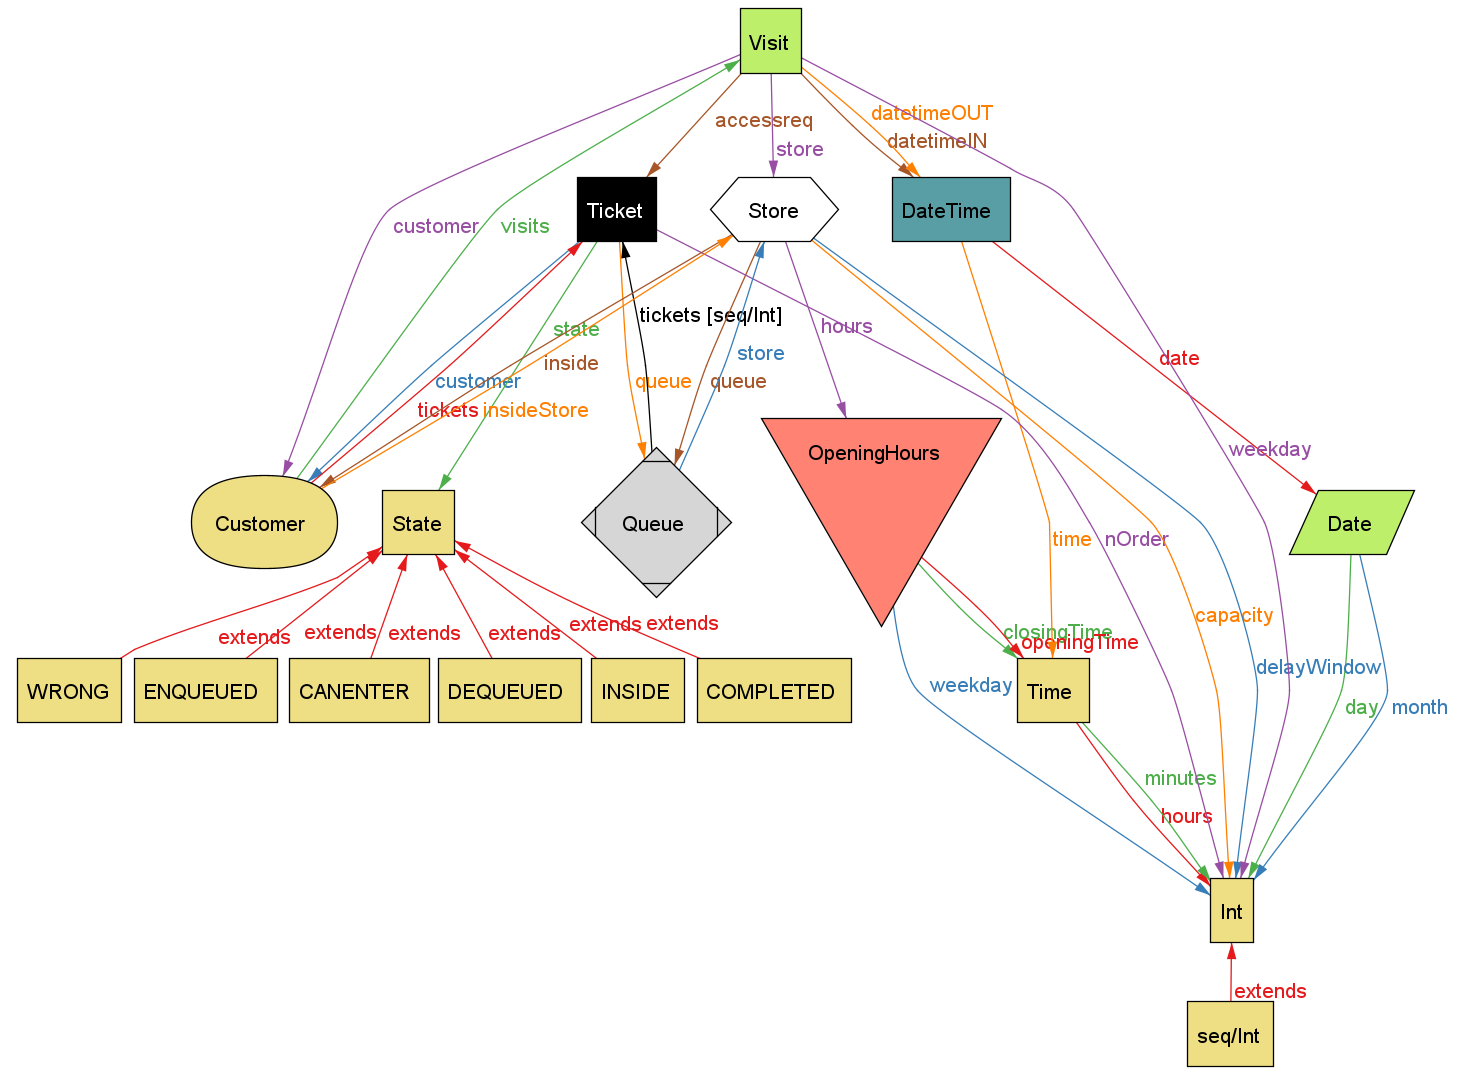
\includegraphics[height=\textheight] {alloy/metamodel}
		\caption{Alloy metamodel}
		\label{metamodel} 
	\end{figure}
	
	\begin{figure}[p]
		\centering	
		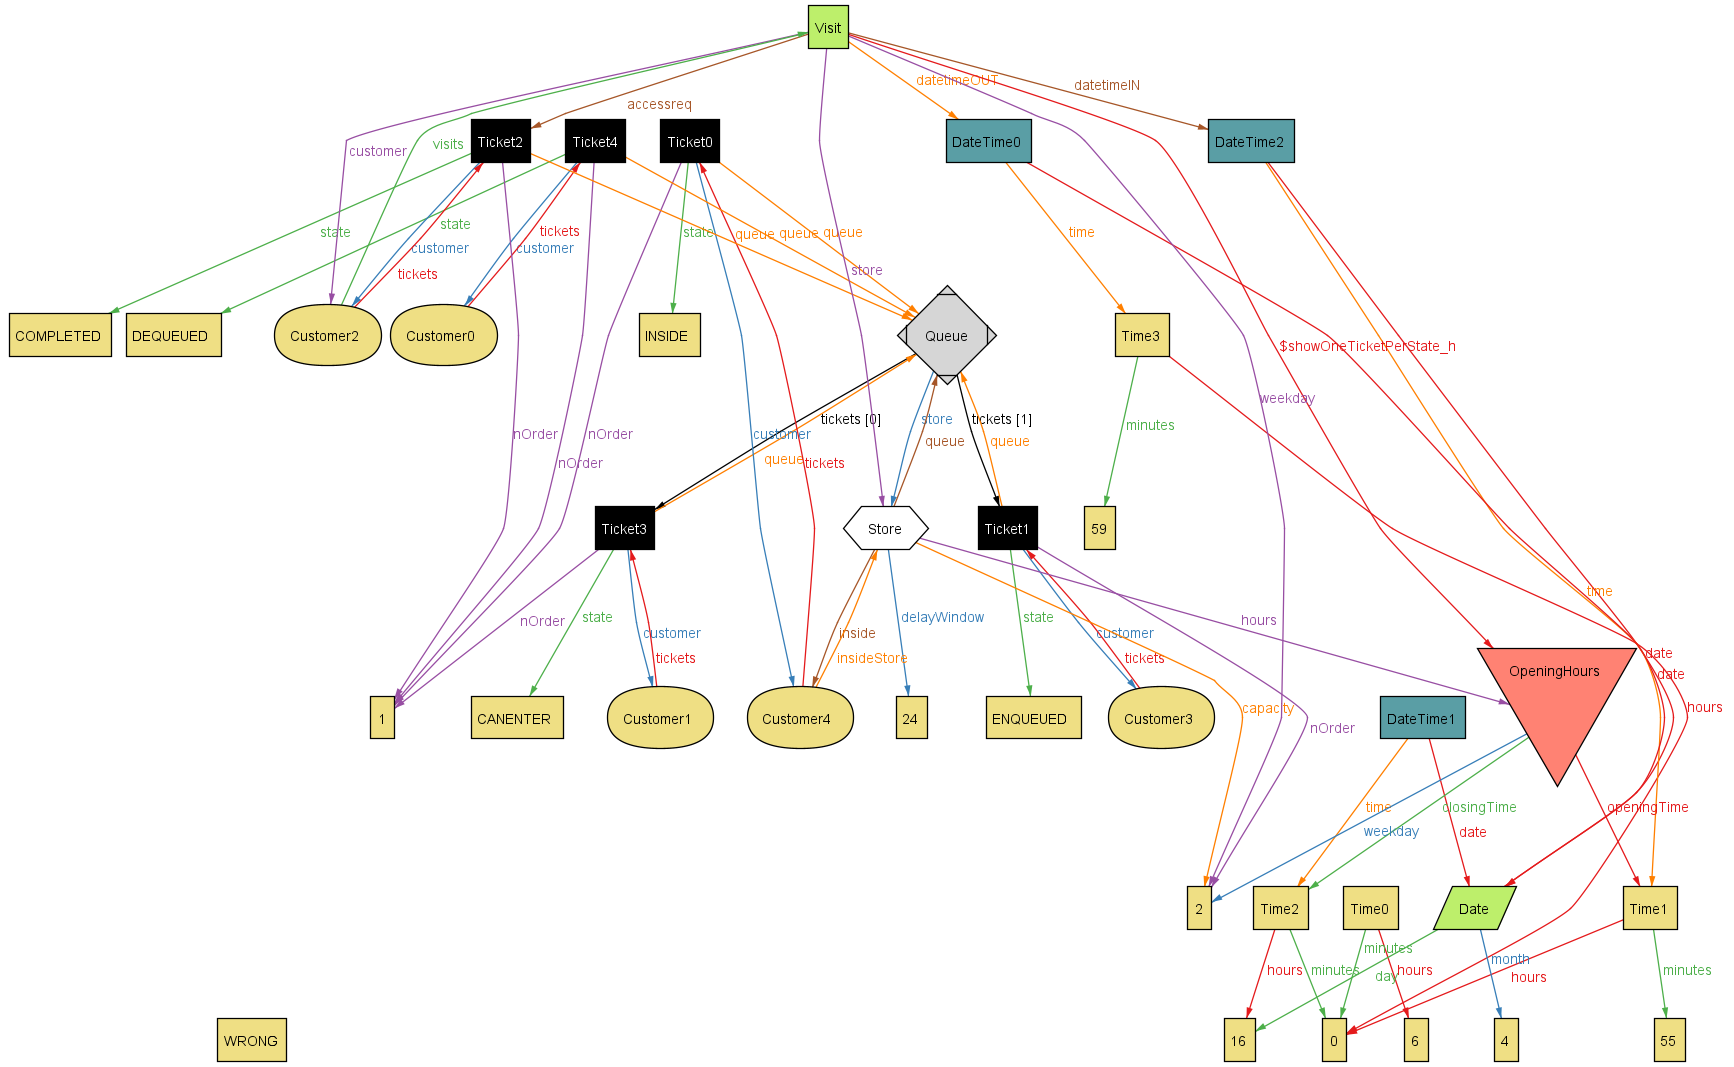
\includegraphics[width=\linewidth] {alloy/1perstate_complete}
		\caption{Result of running \texttt{showOneTicketPerState}}
		\label{oneforstate} 
	\end{figure}
	
	\begin{figure}[p]	
		\centering
		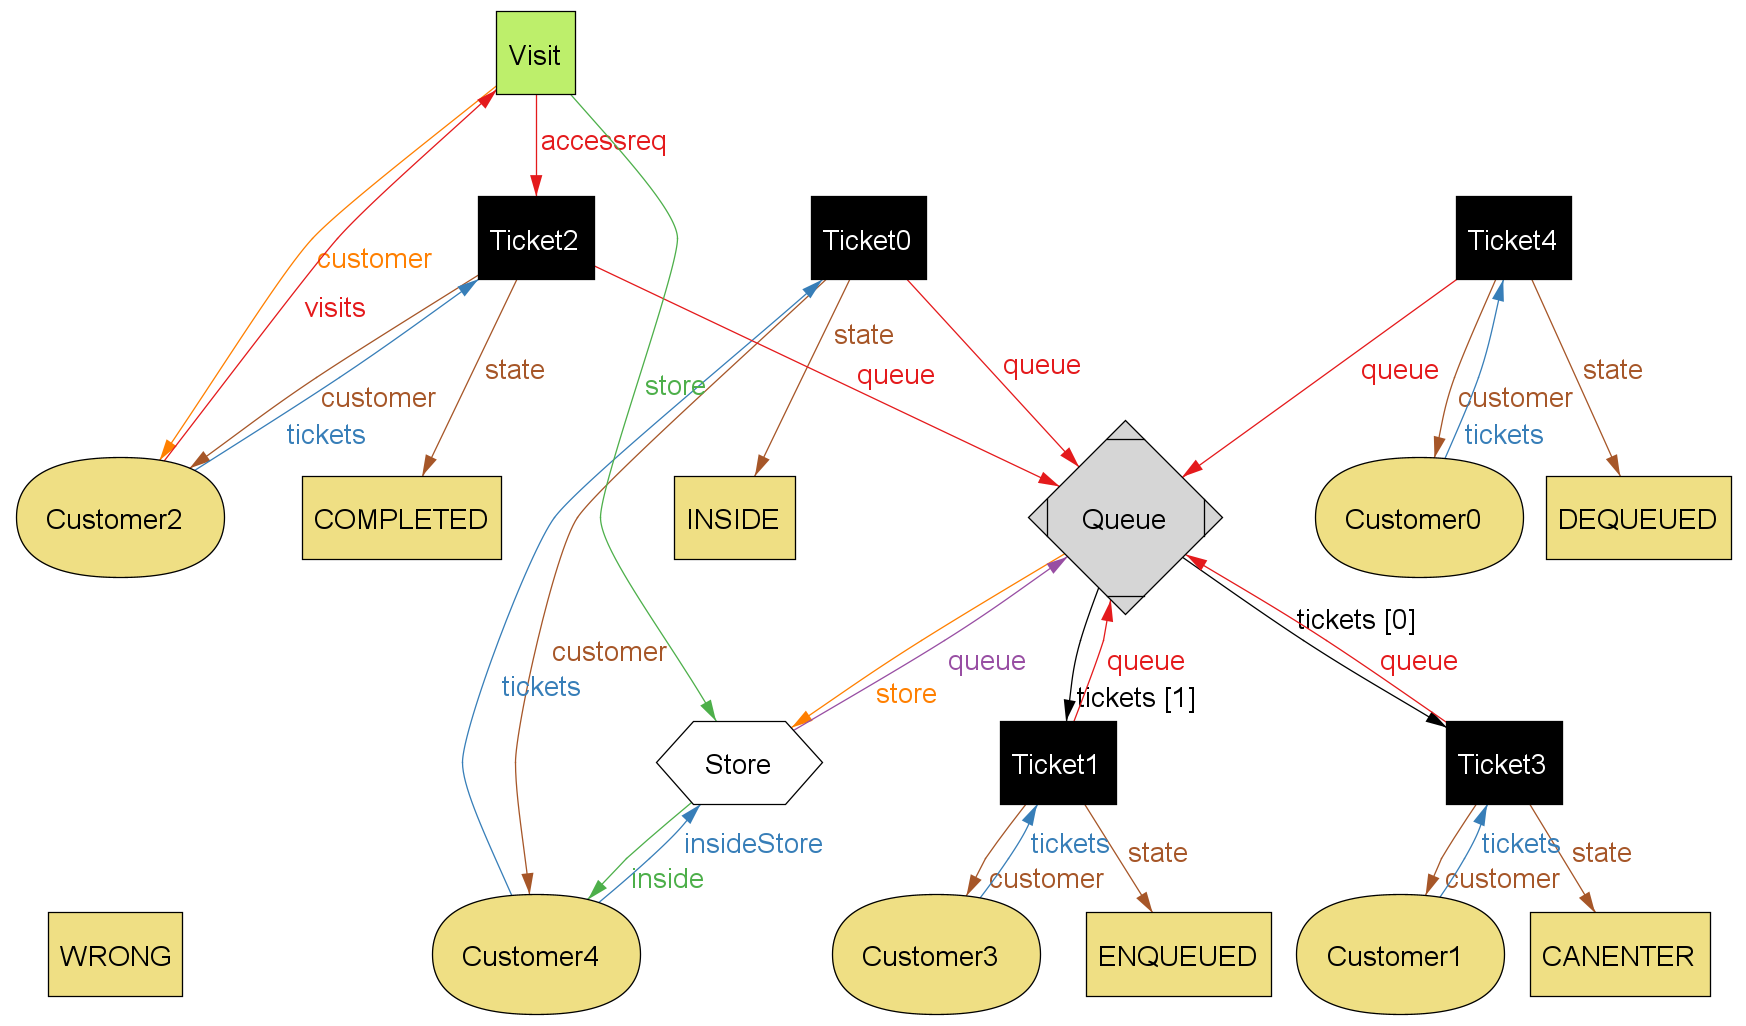
\includegraphics[width=0.8\linewidth] {alloy/1perstate}
		\caption{Result of running \texttt{showOneTicketPerState} (Only relevant signatures)}
		\label{oneforstate_compl} 
	\end{figure}
\end{landscape}
